\documentclass[border=12pt]{standalone}
\usepackage[T1]{fontenc}
\usepackage{helvet}
\renewcommand{\familydefault}{\sfdefault}
\usepackage{amsmath}
\usepackage{tikz}
\usetikzlibrary{positioning,arrows.meta,shapes.geometric,fit,backgrounds,calc,decorations.pathreplacing}

\definecolor{cSetup}{HTML}{34495E}
\definecolor{cOpt}{HTML}{2E6DA4}
\definecolor{cOptBg}{HTML}{EAF2FB}
\definecolor{cQ}{HTML}{C0622A}
\definecolor{cQBg}{HTML}{FBEEE3}
\definecolor{cOut}{HTML}{1E8449}
\definecolor{cLoop}{HTML}{8E44AD}
\definecolor{cInk}{HTML}{1B2631}

\begin{document}
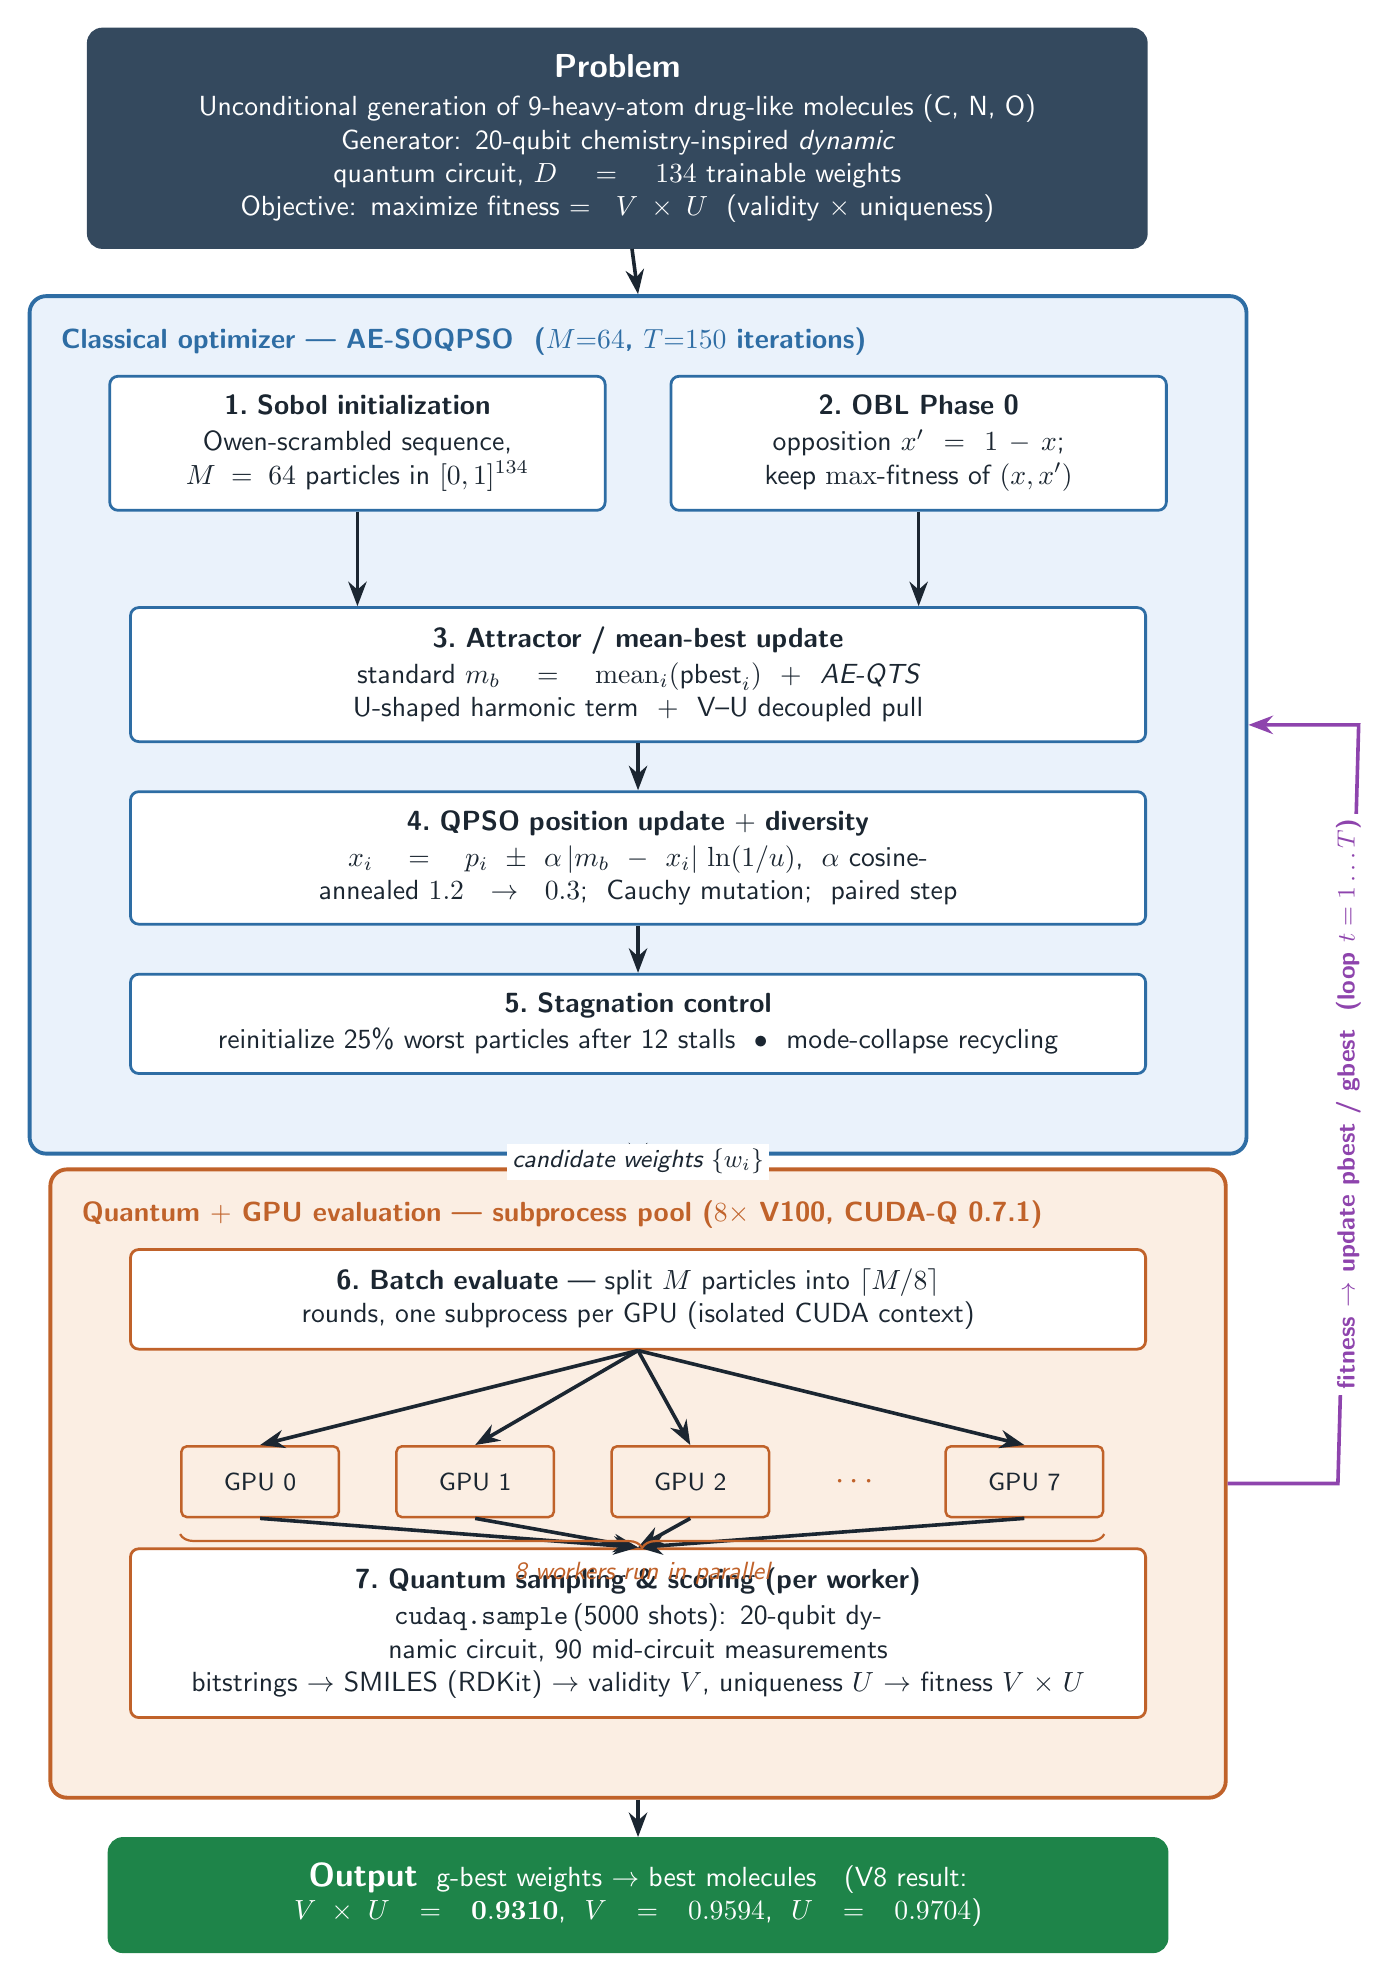
\begin{tikzpicture}[
  font=\sffamily,
  >=Stealth,
  node distance=6mm,
  stage/.style={rectangle, rounded corners=3pt, draw=cOpt, line width=1pt, fill=white,
                text=cInk, align=center, inner sep=7pt, text width=124mm},
  qstage/.style={rectangle, rounded corners=3pt, draw=cQ, line width=1pt, fill=white,
                text=cInk, align=center, inner sep=7pt, text width=124mm},
  half/.style={rectangle, rounded corners=3pt, draw=cOpt, line width=1pt, fill=white,
                text=cInk, align=center, inner sep=7pt, text width=58mm},
  io/.style={rectangle, rounded corners=5pt, draw=#1, line width=1.1pt, fill=#1,
             text=white, align=center, inner sep=9pt, text width=128mm},
  gpu/.style={rectangle, rounded corners=2pt, draw=cQ, line width=0.9pt, fill=cQBg,
              text=cInk, align=center, inner sep=4pt, minimum width=20mm, minimum height=9mm,
              font=\sffamily\small},
  flow/.style={->, line width=1.3pt, draw=cInk},
  loop/.style={->, line width=1.3pt, draw=cLoop},
  elabel/.style={font=\sffamily\small\itshape, text=cInk, fill=white, inner sep=2pt},
  llabel/.style={font=\sffamily\small\bfseries, text=cLoop, fill=white, inner sep=2pt},
  hdr/.style={font=\sffamily\bfseries\normalsize},
]

% ---------- Problem setup ----------
\node[io=cSetup] (setup) {%
  \textbf{\large Problem}\\[2pt]
  Unconditional generation of 9-heavy-atom drug-like molecules (C, N, O)\\
  Generator: 20-qubit chemistry-inspired \emph{dynamic} quantum circuit, $D=134$ trainable weights\\
  Objective: maximize fitness $=V\times U$\ \ (validity $\times$ uniqueness)};

% ---------- Optimizer stages ----------
\node[half, below=16mm of setup.south, xshift=-33mm] (a1)
  {\textbf{1.\ Sobol initialization}\\[1pt] Owen-scrambled sequence,\\ $M=64$ particles in $[0,1]^{134}$};
\node[half, right=8mm of a1] (a2)
  {\textbf{2.\ OBL Phase 0}\\[1pt] opposition $x'=1-x$;\\ keep $\max$-fitness of $(x,x')$};

\node[stage, below=12mm of $(a1.south)!0.5!(a2.south)$] (a3)
  {\textbf{3.\ Attractor / mean-best update}\\[1pt]
   standard $m_b=\mathrm{mean}_i(\text{pbest}_i)$\ \ $+$\ \ \emph{AE-QTS} U-shaped harmonic term\ \ $+$\ \ V--U decoupled pull};
\node[stage, below=of a3] (a4)
  {\textbf{4.\ QPSO position update $+$ diversity}\\[1pt]
   $x_i = p_i \pm \alpha\,|m_b-x_i|\,\ln(1/u)$,\ \ $\alpha$ cosine-annealed $1.2\!\to\!0.3$;\ \ Cauchy mutation;\ \ paired step};
\node[stage, below=of a4] (a5)
  {\textbf{5.\ Stagnation control}\\[1pt]
   reinitialize 25\% worst particles after 12 stalls\ \ $\bullet$\ \ mode-collapse recycling};

% ---------- candidate weights arrow ----------
\node[qstage, below=22mm of a5] (b1)
  {\textbf{6.\ Batch evaluate} --- split $M$ particles into $\lceil M/8\rceil$ rounds,\ one subprocess per GPU (isolated CUDA context)};

% ---------- GPU workers ----------
\node[gpu, below=12mm of b1.south, xshift=-48mm] (g0) {GPU 0};
\node[gpu, right=7mm of g0] (g1) {GPU 1};
\node[gpu, right=7mm of g1] (g2) {GPU 2};
\node[right=7mm of g2, font=\large\bfseries, text=cQ] (gd) {$\cdots$};
\node[gpu, right=7mm of gd] (g7) {GPU 7};

\node[qstage, below=12mm of b1.south, yshift=-13mm] (b3)
  {\textbf{7.\ Quantum sampling \& scoring (per worker)}\\[1pt]
   \texttt{cudaq.sample}\,(5000 shots): 20-qubit dynamic circuit, 90 mid-circuit measurements\\
   bitstrings $\to$ SMILES (RDKit) $\to$ validity $V$, uniqueness $U$ $\to$ fitness $V\times U$};

% ---------- Output ----------
\node[io=cOut, below=15mm of b3] (out)
  {\textbf{\large Output}\ \ g-best weights $\to$ best molecules\quad
   (V8 result: $V\times U=\mathbf{0.9310}$,\ \ $V=0.9594$,\ \ $U=0.9704$)};

% ---------- Panels (background) ----------
\begin{scope}[on background layer]
  \node[rectangle, rounded corners=6pt, fill=cOptBg, draw=cOpt, line width=1.4pt,
        fit=(a1)(a2)(a3)(a4)(a5), inner sep=10mm] (panelA) {};
  \node[rectangle, rounded corners=6pt, fill=cQBg, draw=cQ, line width=1.4pt,
        fit=(b1)(g0)(g7)(b3), inner sep=10mm] (panelB) {};
\end{scope}
\node[hdr, text=cOpt, anchor=north west] at ([xshift=3mm,yshift=-3mm]panelA.north west)
  {Classical optimizer --- AE-SOQPSO\ \ ($M{=}64$, $T{=}150$ iterations)};
\node[hdr, text=cQ, anchor=north west] at ([xshift=3mm,yshift=-3mm]panelB.north west)
  {Quantum $+$ GPU evaluation --- subprocess pool ($8\times$ V100, CUDA-Q 0.7.1)};

% ---------- Arrows ----------
\draw[flow] (setup) -- (panelA.north);
\draw[flow] (a1) -- ($(a1.south)+(0,-12mm)$);
\draw[flow] (a2) -- ($(a2.south)+(0,-12mm)$);
\draw[flow] (a3) -- (a4);
\draw[flow] (a4) -- (a5);
\draw[flow] (panelA.south) -- node[elabel,pos=0.5]{candidate weights $\{w_i\}$} (panelB.north);
\draw[flow] (b1.south) -- (g0.north);
\draw[flow] (b1.south) -- (g1.north);
\draw[flow] (b1.south) -- (g2.north);
\draw[flow] (b1.south) -- (g7.north);
\draw[flow] (g0.south) -- (b3.north);
\draw[flow] (g1.south) -- (b3.north);
\draw[flow] (g2.south) -- (b3.north);
\draw[flow] (g7.south) -- (b3.north);
\draw[decorate,decoration={brace,amplitude=5pt},draw=cQ,line width=0.8pt]
  ([yshift=-2mm]g7.south east) -- ([yshift=-2mm]g0.south west)
  node[midway,yshift=-5mm,font=\sffamily\small\itshape,text=cQ]{8 workers run in parallel};
\draw[flow] (panelB.south) -- (out.north);

% ---------- Feedback loop ----------
\coordinate (rb) at ($(panelB.east)+(14mm,0)$);
\coordinate (ra) at ($(panelA.east)+(14mm,0)$);
\draw[loop] (panelB.east) -- (rb) -- (ra) -- (panelA.east);
\node[llabel, rotate=90] at ($(rb)!0.5!(ra)$) {fitness $\to$ update pbest / gbest\ \ (loop $t=1\ldots T$)};

\end{tikzpicture}
\end{document}
